%!TEX root = ../synopsis.tex

В {\bf первой главе}
проводится анализ проблемы автоматизированного проектирования УП
в раскройно-заготовительном производстве для оборудования термической фигурной резки с ЧПУ.
Описаны основные технологические особенности и ограничения термической резки,
которые необходимо соблюдать при проектировании УП.

В общем случае маршрут инструмента содержит несколько компонент:
начальную и возможно отличную от неё конечную точку маршрута $M_0$ и $M_{N+1}$,
$N$ точек врезки $M_i$, $i \in \overline{1, N}$
и соответствующих им точек выключения инструмента
$M_i^*$,
рабочий ход инструмента от точки врезки $M_i$
до точки выключения $M_i^*$
а также холостой ход от $M_i^*$
до следующей точки врезки $M_{i+1}$,
см. рис.~\ref{fig:toolpath}.
В определение маршрута также входит
порядок резки,
то есть последовательность посещения точек врезки,
представляющая собой перестановку
$I = (i_1, i_2, ... i_N)$.

\begin{figure}[]
  \centering
  \includegraphics[width=0.8\textwidth]{toolpath.pdf}
  \caption{Элементы маршрута резки}
  \label{fig:toolpath}
\end{figure}



\begin{figure}
  \centering
  \includegraphics[width=0.95\textwidth]{classes.pdf}
  \caption{Классификация задач резки}
  \label{fig:cut-classes}
\end{figure}
